\subsection{Several filters: the colour test and TRICERATOPS+}
\label{sec:multiband}

\subsubsection*{Why colour helps}

A planet blocks the same fraction of the starlight in every band; only limb
darkening makes the depth differ by a few per cent between blue and red.
Most false positives do not have that property, because the star that is
eclipsed, or the star that dilutes the dip, has another colour than the
target:

\begin{center}
\begin{tabular}{@{}p{0.26\textwidth}p{0.66\textwidth}@{}}
\toprule
Scenario & Depth versus band\\
\midrule
TP, PTP, DTP (planet) & the same in every band (limb darkening: a few \%)\\
SEB, SEBx2P, STP & the dip is on a bound companion, diluted by the target:
deeper in the band where the companion is relatively brighter (red for a
cooler companion)\\
PEB, PEBx2P & the dip is on the target, diluted by a companion of another
colour: shallower where the companion is brighter\\
BEB, BEBx2P, BTP, DEB, DEBx2P & as above, for an unresolved background or
foreground star of unknown colour\\
NEB, NTP & a resolved neighbour: tested with separate apertures, not with
colours\\
EB, EBx2P & an eclipsing binary on the target: often nearly achromatic;
spectroscopy tests it\\
\bottomrule
\end{tabular}
\end{center}

The farther apart the two bands, the larger the effect: $g'$ with $z'$ (or B
with I) is far better than V with R.

\begin{figure}[ht]
\centering
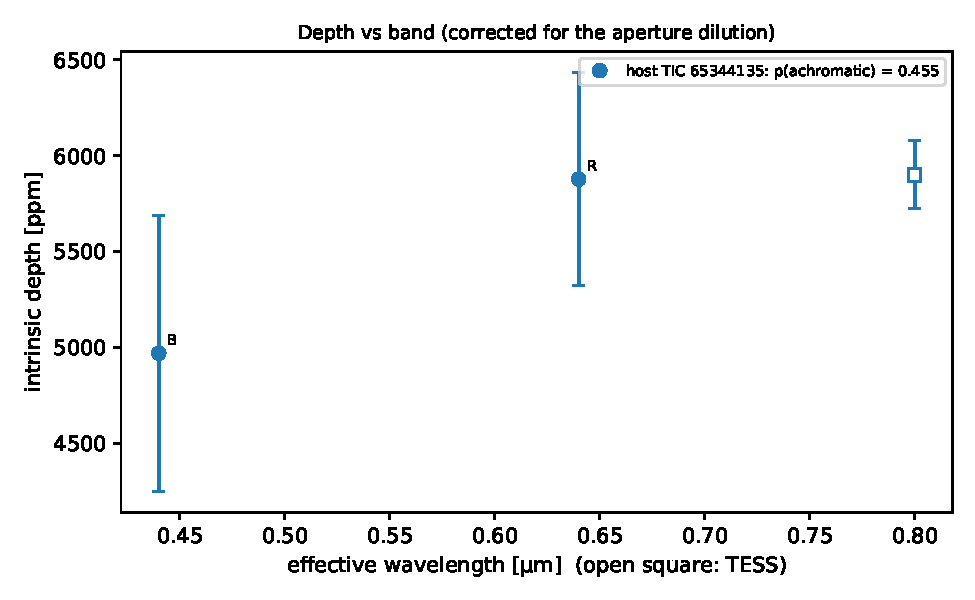
\includegraphics[width=0.62\textwidth]{ground_chromaticity_example.pdf}
\caption[Depth versus band]{\code{ground_chromaticity_<TIC>.pdf} for the synthetic test of
TIC~65344135: the measured depth in each band divided by the target's
flux fraction in that aperture, i.e.\ the intrinsic depth if the target is
the host (dots), and the TESS value (open square). B lies 1.2$\sigma$ below
Rc and TESS; all three agree within their errors ($\chi^2$ test,
$p = 0.46$; see the text).}
\label{fig:gchrom}
\end{figure}

\subsubsection*{Two ways the pipeline uses the bands}

\begin{enumerate}
\item \textbf{TRICERATOPS+.} The extended version of TRICERATOPS
(installed in the \code{triplus} environment) fits the ground light curves
together with TESS. For every scenario it predicts the light curve in each
band, with the band-dependent flux fractions of all stars
(\code{fluxratio_<band>}), and multiplies the likelihoods. The pipeline
passes at most seven light curves, \emph{one per band}: the most precise
usable light curve in each of $g$, $r$, $i$, $z$, $J$, $H$, $K$ (Rc and Ic
count as $r$ and $i$). B, V and clear-filter light curves are not
TRICERATOPS+ bands; they enter only the clearance and the colour test.
With TRICERATOPS+ the reported FPP \emph{already includes} the ground data.
With the original TRICERATOPS (option \code{--tri-plus off}, or another
environment) it does not.
\item \textbf{The colour test.} Independently of TRICERATOPS, the
pipeline converts every ground depth into the intrinsic depth of the host
(dividing by its flux fraction in that aperture and band) and compares the
bands with each other and with TESS (Figure~\ref{fig:gchrom}). Two numbers
summarise the comparison:
\begin{itemize}
\item \emph{$\chi^2$ and $p$.} With $d_k \pm \sigma_k$ the intrinsic depth
in band $k$ (one value per band; TESS included) and $\bar d$ their
error-weighted mean,
\[
\chi^2 = \sum_k \frac{(d_k - \bar d)^2}{\sigma_k^2},
\]
with $n-1$ degrees of freedom for $n$ bands. Each $\sigma_k$ includes a
3~\% systematic floor for the dilution model. The value $p$ is the
probability that a depth which is \emph{the same in every band} would give
a $\chi^2$ at least this large through noise alone (the tail of the $\chi^2$
distribution). A large $p$ means the depths are compatible with an
achromatic dip; the pipeline calls the dip \emph{chromatic} when
$p < 0.0027$, the probability of a 3$\sigma$ deviation. A large $p$ is not
a proof that the dip is achromatic: with large errors every depth
``fits''. That is what the second number is for.
\item \emph{Red/blue ratio.} The ratio of the depths in the reddest and the
bluest band, with its error. Three times that error is the smallest colour
difference these data could have detected.
\end{itemize}
When only one ground band is available, TESS serves as the second band.
\end{enumerate}

\textbf{Reading the example.} The intrinsic depth is $4970 \pm 720$~ppm in
B, $5877 \pm 557$~ppm in Rc and 5900~ppm in TESS. B is lower, but the same
depth was injected in both bands: the difference is noise (the B light
curve is noisier, 2.5 against 2~ppt per point, and its fitted mid-time is
12~min late). The test quantifies this: $\chi^2 = 1.6$ for 2 degrees of
freedom (three bands), $p = 0.46$: a depth that is the same in every band
gives a $\chi^2$ this large or larger in 46~\% of the cases, so it fits; and the ratio
red/blue $= 1.18 \pm 0.21$ is 0.9$\sigma$ from 1. The same number also
shows how weak this pair of light curves is as a colour test: a depth ratio
had to differ from 1 by more than about 60~\% (3$\sigma$) to be detected.
That excludes only strongly chromatic blends; the audit's \emph{Multi-band}
test states this limit (``a colour difference of more than \ldots{} would
have been seen'') and which scenarios it rules out.

\textbf{If the difference were real.} A blue depth significantly below the
red one means that the eclipsed object is redder (cooler) than the light
that dilutes it: for example a transit or eclipse on a cool companion or
background star, diluted by a hotter target (STP, SEB, BEB). A blue depth
above the red one points the other way: a dip on the target diluted by a
redder star. Before concluding either, check the things that also make a
depth depend on the band: comparison stars of very different colour, a
wrong filter name (and so a wrong flux fraction), and differential
extinction during the night. Limb darkening alone changes the depth by only
a few per cent.


\subsubsection*{What the audit says}

The audit test \emph{Multi-band} turns this into a short statement with
the numbers behind it:

\begin{description}
\item[NA] no ground light curves, or fewer than two bands with a measured
depth. The advice says which band to add.
\item[PASS] the depth is the same in every band within the stated limit,
as a planet on the target requires. The audit then lists the scenarios
whose best-fit companion predicts a colour difference the data exclude,
and those it cannot distinguish. Example from the test suite (bands $g$ and
$z$, original TRICERATOPS):
\begin{lstlisting}
PASS  Multi-band  the depth is the same in g and z within 6 % (3 sigma),
  as a planet on the target requires; triceratops is not TRICERATOPS+:
  the ground light curves did NOT enter the FPP; intrinsic depth
  z/g = 1.000 +/- 0.020; ruled out by the colours: SEBx2P (predicts 8.23,
  201 sigma off, P = 0.3); not distinguished: PEB (0.97); removing them
  gives FPP = 0.1429 (the reported FPP does not include the ground data)
  -> run with TRICERATOPS+ (--tri-plus on) so that the light curves
     enter the FPP itself
\end{lstlisting}
\item[WARN / FAIL] the depth depends on the band (more than 3$\sigma$ from
an achromatic depth): the dip is not a planet on the target, or the
dilution in one of the apertures is wrong. It is a FAIL when at least two
bands detect the transit with S/N $\geq 5$. The audit names the scenarios
whose companion reproduces the measured colour.
\end{description}

The page \emph{Next observations} of the audit uses the same calculation
before the observation: for every chromatic scenario it gives the expected
depth ratio between $g'$ and $z'$ and the depth error per band needed to
see it at 3$\sigma$ (Chapter~\ref{ch:followup}).

\subsubsection*{Planning a multi-band observation}

\begin{itemize}
\item \textbf{Bands far apart}, e.g.\ $g'$ and $z'$; simultaneous
observations (two telescopes, or a multi-channel camera) share the same
weather and systematics, which makes the ratio more robust.
\item \textbf{Precision.} A companion of similar colour changes the depth
by only a few per cent. The audit states the limit reached (``within
6~\%''); several transits per band combine.
\item \textbf{Same comparison stars and aperture} in all bands, and the
filter name in the file or in the specification (\code{band=z}); a
wrong filter name gives a wrong flux fraction and a false colour signal.
\item \textbf{Neighbours.} Colours do not replace separate apertures: a
nearby eclipsing binary is found with the clearance test, not with the
colour test.
\end{itemize}
